\documentclass[a4paper]{article}
\usepackage{authblk}
\usepackage[pdftex]{graphicx}
\usepackage{sidecap}
\usepackage[T1]{fontenc}
\usepackage[utf8]{inputenc}
\usepackage[magyar]{babel}
\usepackage{hyperref}
\sloppy
\usepackage{listings}
\lstset{language=C++}

\author[1]{András~Mamenyák}
\author[1]{Roland~Bamli}
\affil[1]{Mérnök informatikus (BSc) szakos hallgató, Debreceni Egyetem}

\title{Neurális hálózatok}

\begin{document}
\maketitle

\section{Bevezetés}
\subsection{A neurális hálózatok kialakulása}
A neurális hálózatok a mesterséges inteligencia egy típusa, amelyet az állatok központi idegrendszere, különösen az agy ihletett, amely képes a tanulásra, a mintafelismerésre is. Megalkotásához biológiai ismeretekre és az idegsejt működésének pontosabb megismerésére volt szükség. Ez csak a 20. században valósult meg. Az első neuron modelt 1947-ben alkotta meg McCullock és Pitts, az első mesterséges neuront pedig Rosenblatt 1958-ban. A neurális hálózatok egy ígéretes, új tudományterület, mely Webos 1974-es "back propagation" algoritmusa és annak 1986-os újra felfedezése után indult igazán fejlődésnek.

\subsection{A mesterséges neuron felépítése, működése}
Egy mesterséges neuron, mint a biológiai, több bemenettel és egy kimenettel rendelkezik (\ref{artifical_neuron}. ábra). Egy általános neuron működése szerint  meghatározza a bemenetek súlyozott összegét és ezen végrehajt valamilyen nem lineáris leképezést. Ez utóbbit nevezik aktivációs, transzfer vagy aktiváló függvénynek. A végeredmény pedig a neuron kimeneti jele. Egy másik változat a lineráris összegzést megvalósító neuron, amikor nem történik lineáris leképezés.

\begin{figure}
  \centering
  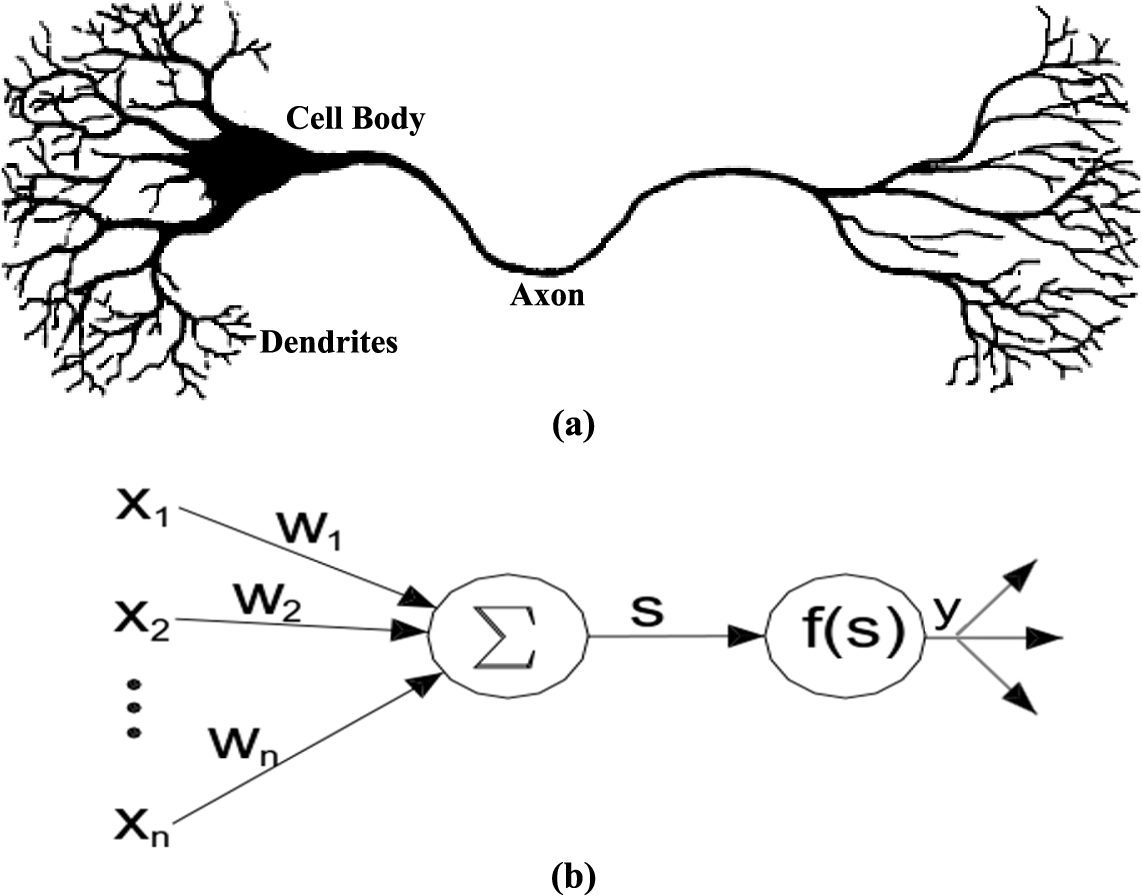
\includegraphics[scale=0.6]{artifical_neuron}
  \caption{A biológiai neuron (a) és a mesterséges neuron (b) összehasonlítása}
  \label{artifical_neuron}
\end{figure}

A \ref{artifical_neuron}. ábrán a neuron bemeneteit x${_i}$ jelöli, a kimeneti jel pedig y. Először a bemenetek súlyozott összegei kerülnek meghatározásra: $${s=\sum_{i=0}^{n} W_i \cdot x_i = W^T \cdot x}$$

Abban az esetben, ha a neuron lineáris összegzést valósít meg, ezzel már meg is kaptuk a kimeneti jelet:$${y = s = W^T \cdot x}$$

Nem lineáris esetben szükség van még a nem lineáris leképezésre. Ebben az esetben a neuron kimeneti jele a következő:$${y = f(s) = f(W^T \cdot x)}$$ ahol ${f(s)}$ az aktivizációs függvény. Erre a célra a négy leggyakrabban használt függvény a lépcső- vagy szignumfüggvény, a ``telítéses lineáris'' függvény, a tangens hiperbolikusz függvény és a szigmoid függvény.

Használnak egy másik elterjedt neuron típust is a RBF (Radial Bass Function) hálózatokban. Ennél a típusnál nincs lineáris összegzés,  az összes bemenet az aktivizációs függvénybe kerül, mely több bemenet esetén több változós függvény lesz.

\subsection{A neuron hálózatok felépítése}
A neuronokból álló hálózatokat nevezzük neurális hálózatoknak. Ezekben minden neuron ugyanolyan, vagy hasonló műveleteket végez, a többi neurontól függetlenül, lokálisan. Tehát ezek a hálózatok olyan információfeldolgozó eszközök, amelyek párhuzamos, elosztott működésre, tanulásra képesek. Általában irányított gráffal reprezentáljuk őket. A neuronok a gráf csomópontjai, míg a gráf élei a kimenetek és bemenetek közötti kapcsolatot reprezentálják. Megvalósíthatók szoftveresen, hardveresen, vagy a kettő kombinációjaként is. 

A neuronok három fajtáját különböztetjük meg:
\begin{enumerate}
    \item\textbf{bemeneti neuronok:} Egy bemenetű, egy kimenetű, buffer jellegű neuronok, jelfeldolgozó feladatuk nincs. Bemenetük a hálózat bemenete, kimenetük más neuronok meghajtására szolgál.
    \item\textbf{rejtett neuronok:} Ezek a neuronok végzik a jelfeldolgozást. Kimenetük és bemenetük is más neuronokhoz csatlakozik.
    \item\textbf{kimeneti neuronok:} A környezet felé továbbítják kimenetüket.
\end{enumerate}

A neuronokat álltalában típusa alapján rétegekbe szervezzük. Ennek megfelelően beszélhetünk bemeneti rétegről, retjett réteg(ek)ről és kimeneti rétegről.

A neuronhálózatokat az egyes neuronok közötti összeköttetési rendszer alapján két fő csoportba sorolhatjuk. Beszélhetünk előrecsatol hálózatokról (\ref{forward_neuron}. ábra) és visszacsatolt hálózatokról. Akkor nevezünk egy neurálos hálózatot visszacsatoltnak, ha a topológiáját reprezentáló irányított gráf tartalmaz hurkot. Ez esetben beszélhetünk globális és lokális visszacsatolásról.

\begin{figure}
  \centering
  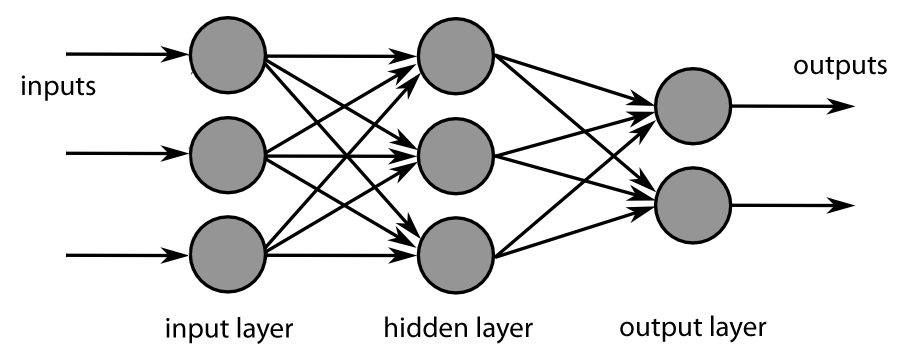
\includegraphics[scale=0.3]{neuron_layers}
  \caption{Előrecsatolt neuron hálózatok felépítése.}
  \label{forward_neuron}
\end{figure}

\subsection{Back-propagation algoritmus}
A back-propagation, teljes nevén ``backward propagation of errors'', magyarul hiba-visszaterjesztési eljárás, egy tanulási algoritmus, melyet gyakran használnak a neurális hálózatokban. Ez egy felügyelt tanulási módszer, melynek szüksége van egy nagy adatbázisra a bemenetekkel és a kívánt kimenetekkel. Alkalmazása az előrecsatolt hálózatoknál a leghasznosabb. Használatához meg kell követelnünk, hogy a neuron hálózat réteges felépítésű, a neuron átviteli függvénye pedig deriválható legyen. Az algoritmusban a tanulás lényegében a hátrafelé terjedés folyamata, mely során minimalizálni kell az elvárt és a tényleges output vektor közötti négyzetes eltérést, Euklideszi távolságot.

Működése alapján két fázisra lehet osztani, terjedésre (propagation) és a súlyok frissítésére. A terjedés során a jel mind előre, mind hátra a szinapszisok és a neuronok szintjén lokális információk alapján terjed. A súlyok frissítése a neuron kimenetére visszaérkezett jel alapján történik (\ref{backpropagation}. ábra).

\begin{figure}
  \centering
  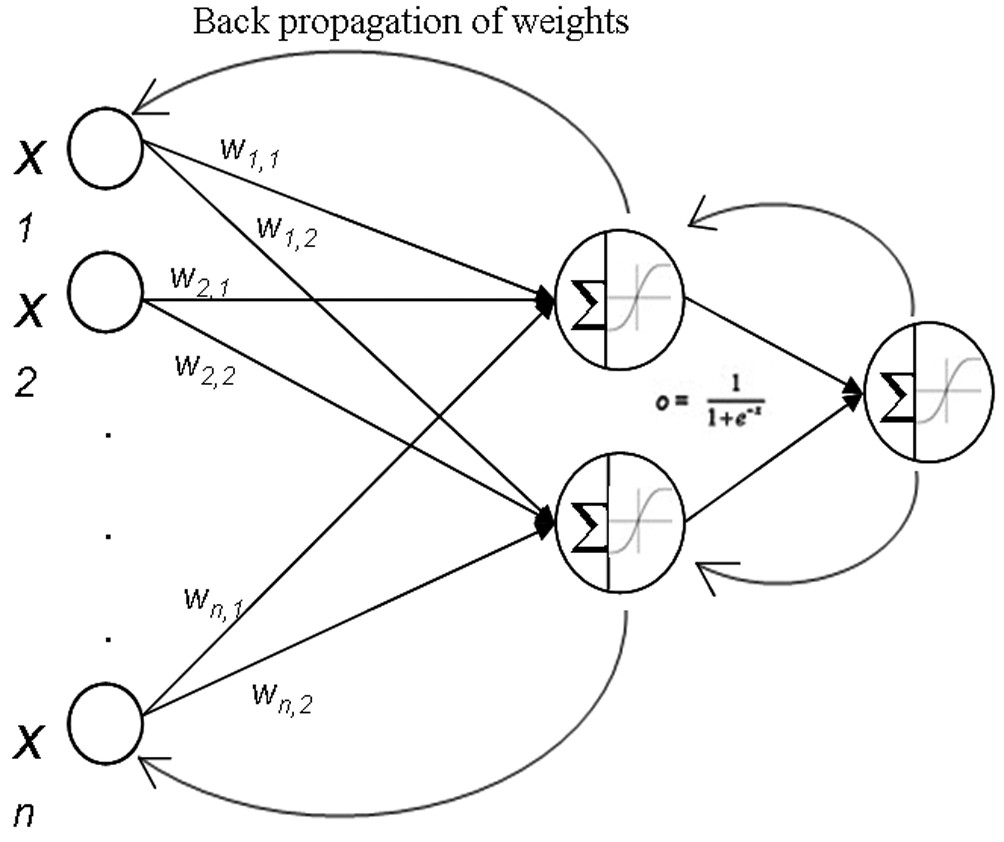
\includegraphics[scale=0.8]{backpropagation}
  \caption{A back-propagation algoritmus működése.}
  \label{backpropagation}
\end{figure}

\section{Az algoritmus implementálása}
Egy neurális háló beprogramozása sok időt vehet igénybe és fölösleges. Ezért egy, már készen levő neurális hálót fogunk alkalmazni a Barker kód teszteléséhez. A szerző az alábbi megjegyzéssel tette közzé a C++ forráskódot:

\lstinputlisting{NEURALI.CPP}

A kód önmagában nem működött, először fordítási hibát kaptunk, majd azt kijavítva ``segmentation fault'' hibával szállt el. A hiba forrása a ``Network'' osztály destruktora:

\begin{lstlisting}
\\ segmentation fault
~Network()
{
  delete Layers;
}

\\ helyesen
~Network()
{
  delete[] Layers;
}
\end{lstlisting}

Az eredeti program több más sebből is vérzett, de kisebb-nagyobb módosításokkal, átszervezéssel sikerült alap esetben a futási időt 25\%-val lecsökkenteni.
Természetesen másfajta, nem programozási módosításokra is szükség volt, hogy a célnak megfelelő neurális hálót kapjunk. A Barker kód 11 bitet feleltet meg 1 bitnek, ezért a neurális hálónknak 11 bemeneti neuronja, 11 rejtett neuronja és 1 kimenei neuronja van.

A végső forrás kód:

\lstinputlisting{neural.cpp}

\section{A program futtatása és a kimenet értelmzése}

A program fordítása és futtatása az alábbi módon végezhető el:

\lstset{language=Bash}
\begin{lstlisting}
andras@G53SW:~/Programs/Neural$ g++ neural.cpp -o neural
andras@G53SW:~/Programs/Neural$ ./neural
\end{lstlisting}

\lstinputlisting{output}

A neurális hálót

\lstset{language=C++}
\begin{lstlisting}
  const int Niter = 10000;
\end{lstlisting}
iteráción keresztül ``tanítattjuk'', mindegyik esetben ugyanazt a
\begin{lstlisting}
  const int Ntrain = 256;
\end{lstlisting}
random bemeneti adatot és a hozzájuk tartozó kimeneti értéket tápláljuk a neurális hálóba. Ez alapján állítódnak be az egyes neuronokhoz tartozó súlyok, amik kezdetben random értékek voltak. Ezután az éles tesztben ráengedjük mind a $2^{11}$ esetet és amint a fenti kimenetben látható, csupán 15 esetben lépte át a kimenet értéke a $0.5$-öt. A várt $11100010010$ ($1811$)-as értékre kaptuk a legjobb eredményt, $0.987942$-t. Ebből jól látható, hogy a neurális hálónk megfelelően működik, megtanulta melyik a Barker kód, és csak nagyjából 1 bitben különböző bemenetekre ad magasabb kimeneti értéket.

\section{Az algoritmus finomhangolása}
Sok állítható paraméterrel rendelkezik az algoritmusunk, ezért számos beállítással kipróbáltuk. A cél az volt, hogy a legnagyob pontosságot érjük el viszonylag rövid futási időn belül. Ha az iterációk számát növeltük, lineárisan növekedett a futási idő is, viszont az eredmény nem lett sokkal pontosabb. Ugyanez érvényes a bemeneti adatok számára is. A legnagyobb különbséget a rejtett neuronok számának növelése jelentette, így értük el optimális futási idő alatt

\lstset{language=Bash}
\begin{lstlisting}
real	0m7.484s
user	0m7.463s
sys	0m0.014s
\end{lstlisting}

a megfelelő pontosságot.

\section{Konklúzió}
A projekt során a ma népszerű kutatási területnek számító neurális hálózattal foglalkoztunk. Megismerkedtünk az alapvető felépítésével és működésével ezekenek a gépi tanulást végző rendszereknek, valamint sikerült a Barker 11 kódot helyesen tesztelő programot készítetnünk.

A program letölthető a \url{https://github.com/mamenyaka/Neural} github tárolóból.

\end{document}